\chapter{Introduzione ai Sistemi Embedded}
Questo capitolo introduce i concetti fondamentali, l'evoluzione storica e i vincoli di progettazione dei sistemi embedded. Vengono approfondite le differenze architetturali tra microprocessori e microcontrollori, analizzando il ruolo discriminante della MMU e la gerarchia delle memorie. Infine, vengono esaminati i principali paradigmi software, dai modelli Foreground-Background ai sistemi operativi Real-Time e Linux Embedded, fino ai requisiti di ingegnerizzazione per la transizione dal prototipo al prodotto finito.

\section{Definizione e Caratteristiche dei Sistemi Embedded}
Un sistema embedded è un dispositivo di calcolo a microprocessore o microcontrollore integrato all'interno di un sistema fisico più ampio, progettato per svolgere un'attività specifica o un insieme ben definito di compiti strettamente correlati. A differenza dei sistemi di calcolo General-Purpose, l'utente finale non ha la facoltà di installare, rimuovere o modificare le applicazioni software.

I sistemi informatici si dividono nelle seguenti categorie:
\begin{itemize}
    \item \textbf{Sistemi General-Purpose} $\rightarrow$ calcolatori destinati a un'ampia classe di applicazioni eterogenee, programmabili dall'utente finale e orientati a massimizzare la velocità media di calcolo secondo il criterio per cui una maggiore velocità corrisponde a un sistema migliore (es. personal computer, laptop, server, mainframe).
    \item \textbf{Sistemi Embedded} $\rightarrow$ dispositivi monofunzionali o a funzionalità dedicata, integrati all'interno dell'ambiente di lavoro con minimo intervento dell'operatore.
    \item \textbf{Sistemi Real-Time} $\rightarrow$ piattaforme in cui la correttezza della risposta è vincolata al rispetto di scadenze temporali certe, non necessariamente coincidenti con sistemi embedded.
    \item \textbf{Sistemi Embedded Real-Time} $\rightarrow$ sistemi embedded dedicati operanti sotto vincoli temporali stringenti di reazione e determinismo.
\end{itemize}

I dispositivi convenzionali quali personal computer e smartphone non costituiscono device embedded in quanto non sono dedicati a una singola attività, permettono l'esecuzione contemporanea o sequenziale di molteplici programmi applicativi a discrezione dell'utente e presentano un'interazione utente continua e non predefinita.

I sistemi embedded sono caratterizzati da specifici attributi architetturali e funzionali:
\begin{itemize}
    \item \textbf{Monofunzionalità} $\rightarrow$ esecuzione ripetitiva di una singola funzione specifica o di un insieme molto ristretto di attività correlate, ottimizzate sulle peculiarità dell'hardware.
    \item \textbf{Interazione minima con l'utente} $\rightarrow$ operatività automatizzata con interventi ridotti o assenti da parte dell'operatore umano.
    \item \textbf{Vincoli progettuali stringenti} $\rightarrow$ requisiti rigidi in termini di costo ridotto (low cost), consumo energetico minimo (low power), ingombro dimensionale compatto (small size) e semplicità di utilizzo.
    \item \textbf{Operatività continua e non presidiata} $\rightarrow$ funzionamento prolungato nel tempo (24/7) senza necessità di supervisione, con elevatissimi standard di affidabilità e robustezza.
\end{itemize}

Dal punto di vista funzionale, il sistema embedded costituisce una \textit{combinazione su misura di componenti hardware e software reattiva e vincolata nel tempo rispetto all'ambiente operativo circostante}. Il dispositivo riceve informazioni dal \textit{processo esterno} attraverso una serie di \textit{sensori}, elabora i dati acquisiti e agisce direttamente sull'ambiente tramite \textit{attuatori}, interfacciandosi all'occorrenza con un'\textit{interfaccia uomo-macchina}.
\begin{figure}[H]
	\centering
	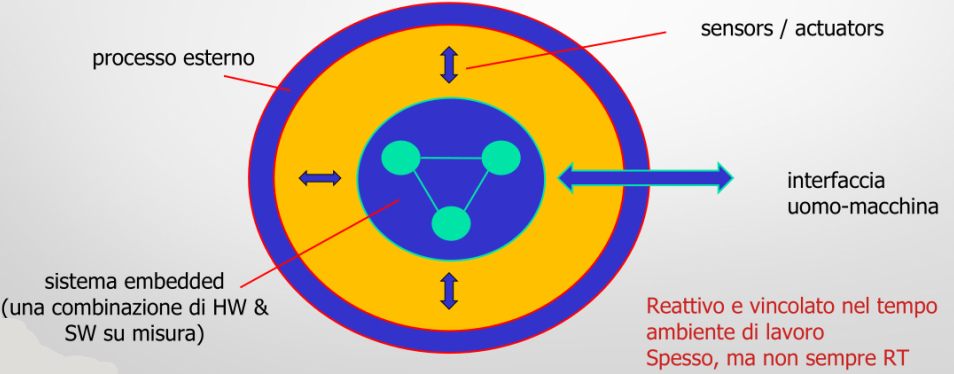
\includegraphics[width=0.7\linewidth]{immagini/introduzione}
\end{figure}

I campi di applicazione dei sistemi embedded comprendono molteplici settori dell'ingegneria e dell'industria:
\begin{itemize}
    \item \textbf{Elettronica di consumo} $\rightarrow$ lettori MP3, altoparlanti wireless, auricolari, dispositivi indossabili, periferiche per personal computer, telecomandi, ricevitori televisivi non smart, accessori dedicati per smartphone.
    \item \textbf{Elettrodomestici} $\rightarrow$ forni a microonde, lavatrici, frigoriferi, impianti di condizionamento, caldaie, centraline di sicurezza domestica.
    \item \textbf{Automazione d'ufficio} $\rightarrow$ apparati di connessione modem, stampanti, scanner.
    \item \textbf{Attrezzature aziendali} $\rightarrow$ impianti di allarme antintrusione, terminali per punti vendita (POS).
    \item \textbf{Automotive} $\rightarrow$ centraline di iniezione elettronica, sistemi di frenata antibloccaggio.
    \item \textbf{Avionica, Aerospazio e Trasporti} $\rightarrow$ sistemi di navigazione satellitare e inerziale, strumentazione di bordo, piattaforme Digital Fly-By-Wire per aeromobili, treni e sottomarini.
    \item \textbf{Medicina} $\rightarrow$ sistemi di supporto vitale, dispositivi medici impiantabili, strumentazione di diagnostica clinica e monitoraggio, apparati di telemedicina.
    \item \textbf{Telecomunicazioni} $\rightarrow$ commutatori di rete, router, apparati di ricetrasmissione modem LTE.
    \item \textbf{Automazione industriale} $\rightarrow$ sistemi di monitoraggio ambientale e di processo, manipolatori robotici e controllori di asse.
\end{itemize}

\section{Evoluzione Storica dei Sistemi Embedded}
L'origine dei sistemi dedicati risale alla fine degli anni '40 con lo sviluppo del calcolatore MIT Whirlwind, espressamente concepito per la simulazione del comportamento dinamico e delle reazioni di volo di un aeromobile in tempo reale.
\begin{figure}[H]
	\centering
	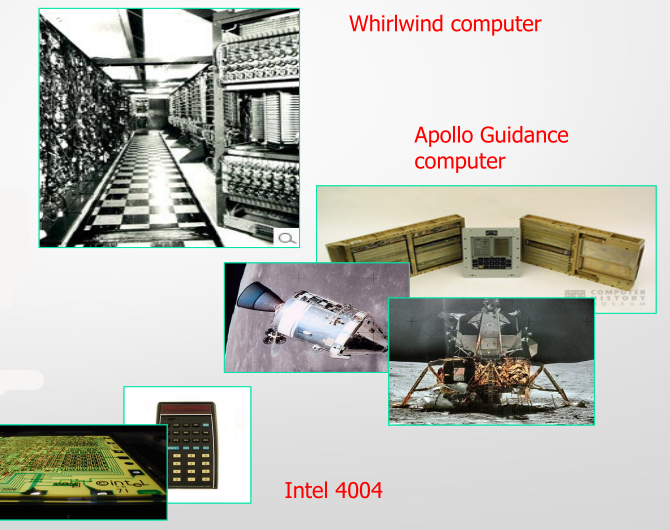
\includegraphics[width=0.55\linewidth]{immagini/introduzione1}
\end{figure}
Negli anni '60 venne realizzato il primo sistema embedded universalmente riconosciuto: l'Apollo Guidance Computer, progettato dal MIT Instrumentation Laboratory per gestire in autonomia la navigazione, il calcolo della traiettoria e il controllo del modulo di comando e del modulo lunare del programma Apollo.

Alla fine degli anni '80, con l'avvento dei microprocessori a singolo circuito integrato (inaugurati dal componente Intel 4004), i sistemi embedded hanno smesso di rappresentare un'eccezione tecnologica per trasformarsi nello standard operativo della quasi totalità degli apparati elettronici.

Nei sistemi attuali, l'architettura embedded ha assunto una struttura complessa basata su reti eterogenee di processori distribuiti, in grado di eseguire sistemi operativi standard e di comunicare attraverso bus cablati (come i bus di campo industriali e automobilistici), reti wireless, reti LAN e WAN. All'interno di un'automobile moderna di fascia alta possono essere presenti fino a circa 100 processori dedicati, ripartiti gerarchicamente per compiti:
\begin{itemize}
    \item Microcontrollori a 4 bit dedicati a funzioni ausiliarie elementari, come il blocco e il pretensionamento delle cinture di sicurezza.
    \item Microcontrollori a 16 bit preposti alla gestione degli strumenti e degli indicatori del cruscotto.
    \item Microcontrollori o processori a 16 e 32 bit per la centralina di controllo motore (ECU).
    \item Processori a 32 e 64 bit dedicati all'elaborazione grafica e multimediale dei sistemi di infotainment di bordo.
\end{itemize}
\begin{figure}[H]
	\centering
	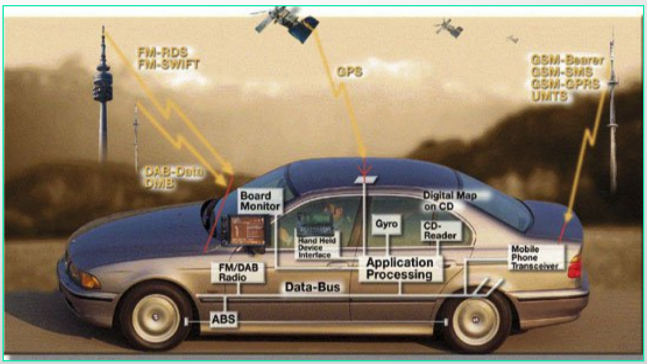
\includegraphics[width=0.55\linewidth]{immagini/introduzione2}
\end{figure}


\section{Metodologia di progettazione e vincoli di sistema}
La progettazione di un sistema embedded adotta un approccio flessibile e iterativo, in cui le fasi preliminari di specifica dei requisiti avvengono spesso contemporaneamente alla stesura dell'architettura hardware e software:
\begin{enumerate}
    \item \textbf{Analisi dei requisiti} $\rightarrow$ identificazione dettagliata del contesto operativo in cui il dispositivo deve operare, definizione delle funzionalità da svolgere e degli obiettivi prestazionali richiesti.
    \item \textbf{Codesign Hardware/Software} $\rightarrow$ ripartizione delle funzioni tra silicio ed elaborazione logica, selezione della piattaforma di calcolo (microcontrollore o microprocessore in funzione di frequenza di clock, memoria e MIPS necessari), identificazione del corredo di periferiche e scelta dell'ambiente software (architettura Foreground-Background, RTOS minimale o sistema operativo completo).
\end{enumerate}

Essendo progettato per essere special-purpose, un sistema embedded deve garantire la massima efficienza nell'esecuzione continua delle sue specifiche mansioni, rispettando rigorosi vincoli costruttivi:
\begin{itemize}
    \item Elevata efficienza energetica con minimizzazione dei consumi (low power), fondamentale per apparati alimentati a batteria o privi di manutenzione.
    \item Costi computazionali contenuti, evitando sovradimensionamenti hardware ingiustificati.
    \item Basso footprint di memoria (quantità di memoria che un programma utilizza durante la sua esecuzione), con allocazione ottimizzata sia per il codice di programma sia per le strutture dati.
    \item Ridotto ingombro dimensionale e peso limitato, requisiti imprescindibili per applicazioni inserite all'interno di dispositivi portatili, veicoli o apparati medici quali i pacemaker.
\end{itemize}

L'affidabilità (reliability) costituisce un parametro cardine di valutazione, misurato quantitativamente attraverso due metriche fondamentali:
\begin{itemize}
    \item \textbf{MTTF} (Mean Time To Failure) $\rightarrow$ tempo medio intercorrente fino al manifestarsi di un guasto permanente, che deve essere massimizzato.
    \item \textbf{MTTR} (Mean Time To Repair) $\rightarrow$ tempo medio necessario alla riparazione o ripristino della piena operatività, che deve essere minimizzato.
\end{itemize}

Il sistema deve inoltre soddisfare requisiti di sicurezza declinati nella duplice dimensione di:
\begin{itemize}
    \item \textbf{Safety} $\rightarrow$ protezione da guasti accidentali, rischi operativi e malfunzionamenti fortuiti, garantendo che il dispositivo non arrechi in alcuna condizione danni fisici agli utenti o all'ambiente circostante.
    \item \textbf{Security} $\rightarrow$ protezione attiva contro minacce informatiche e attacchi deliberati, assicurando la riservatezza, l'integrità delle informazioni e l'accesso ai soli soggetti o processi esplicitamente autorizzati.
\end{itemize}

\section{Sistemi Real-Time}
Nei sistemi embedded, l'affidabilità è strettamente correlata alla \textbf{reattività}, definita come l'attitudine del sistema a elaborare e rispondere agli stimoli provenienti dall'ambiente esterno entro finestre temporali precise.

Il termine Real-Time trae la propria origine dalle prime simulazioni di volo e di processi complessi, in cui la simulazione procedeva a una velocità coincidente con quella dell'evento fisico reale simulato. In base al comportamento temporale, i sistemi informatici si distinguono in tre macro-categorie:
\begin{itemize}
    \item \textbf{Sistemi Batch} $\rightarrow$ elaborazioni in cui non sussiste alcuna scadenza operativa vincolante tra l'insorgenza dell'evento e la produzione della risposta (es. esecuzione di una stored procedure SQL).
    \item \textbf{Sistemi Interactive On-line} $\rightarrow$ contesti in cui un tempo di risposta rapido è auspicabile per migliorare l'usabilità, ma non condiziona la correttezza logica del risultato (es. sistemi operativi desktop convenzionali).
    \item \textbf{Sistemi Real-Time} $\rightarrow$ sistemi in cui la risposta deve essere erogata inderogabilmente entro un intervallo temporale prestabilito, pena il fallimento del sistema stesso.
\end{itemize}

Un sistema Real-Time non è necessariamente un sistema embedded. In relazione alla severità del vincolo temporale (deadline), si individuano due tipologie di funzionamento:
\begin{itemize}
    \item \textbf{Hard Real-Time} $\rightarrow$ il rispetto della scadenza temporale (deadline) è assoluto e tassativo. Il mancato completamento del calcolo o dell'azione entro il limite stabilito equivale al collasso del sistema e può comportare danni catastrofici a beni, operatori o ambiente circostante. Tipicamente associati a una complessità software contenuta, i sistemi Hard Real-Time non sono semplicemente sistemi veloci, bensì sistemi certificati per garantire tempi di intervento deterministici e certi.
    \item \textbf{Soft Real-Time} $\rightarrow$ la presenza di una finestra di tolleranza ammette ritardi occasionali nella risposta; il superamento della scadenza non pregiudica l'incolumità delle persone né l'integrità dell'ambiente, comportando unicamente un degrado delle prestazioni fornite.
\end{itemize}

Un esempio primario di applicazione Hard Real-Time è costituito dal sistema di attivazione dell'airbag nei veicoli a motore, in cui il rilevamento della collisione e il comando di innesco devono avvenire rigorosamente entro una frazione di millisecondo prefissata.
\begin{figure}[H]
	\centering
	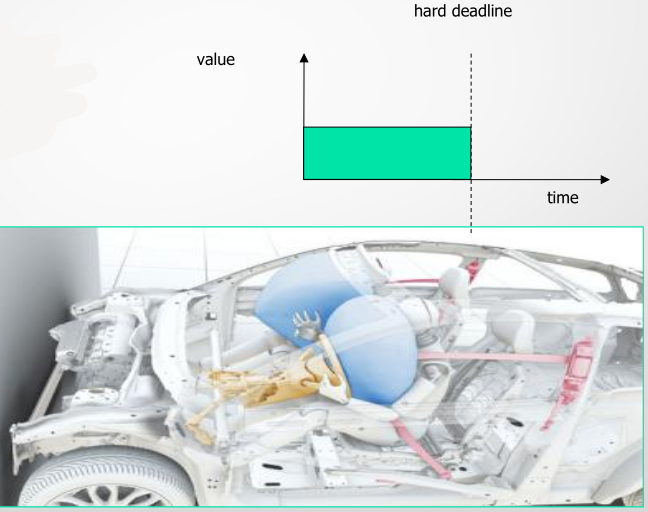
\includegraphics[width=0.5\linewidth]{immagini/introduzione3}
\end{figure}

\section{Distinzione tra Software e Firmware}
Il concetto di firmware è intrinsecamente legato al settore dei sistemi embedded e dei microcontrollori. Il termine identifica la frazione del codice software posizionata a più stretto contatto con l'hardware fisico sottostante.

Più formalmente, il firmware è l'insieme delle istruzioni residenti permanentemente all'interno della memoria non volatile del dispositivo, preposte a inizializzare, controllare e alimentare l'hardware specifico destinato all'applicazione.

Sul piano pratico e metodologico si individua una netta demarcazione di impiego:
\begin{itemize}
    \item \textbf{Software} $\rightarrow$ associato all'ambiente di calcolo General-Purpose, caratterizzato da livelli di astrazione elevati, portabilità tra diverse macchine e gestione tramite sistema operativo.
    \item \textbf{Firmware} $\rightarrow$ associato all'architettura dei microcontrollori, sviluppato su misura per pilotare direttamente registri e periferiche della piattaforma embedded senza intermediari astratti.
\end{itemize}
Tipicamente su un microcontrollore non girano dei software, ma è possibile farlo in alcuni casi. Ad esempio, quando si necessitano librerie grafiche o di rete si può caricare un sistema operativo sul microcontrollore per evitare di scrivere manualmente dei driver.

\section{Microprocessori e Microcontrollori}
Le unità di elaborazione utilizzate nell'elettronica digitale comprendono diverse famiglie di dispositivi:
\begin{itemize}
    \item \textbf{General-Purpose Processors (GPP o CPU)} $\rightarrow$ unità centrali di elaborazione destinate all'informatica generale e a compiti computazionali complessi.
    \item \textbf{Microcontrollori (MCU)} $\rightarrow$ dispositivi integrati su singolo chip orientati al controllo diretto di sistemi fisici e periferiche.
    \item \textbf{Digital Signal Processor (DSP)} $\rightarrow$ processori specializzati nell'elaborazione numerica real-time di segnali analogici digitalizzati.
    \item \textbf{Advanced RISC Machine (ARM)} $\rightarrow$ famiglie di processori basati su architettura RISC, scalabili da microcontrollori a processori applicativi ad alte prestazioni.
\end{itemize}

\subsubsection{Microprocessore General-Purpose}
Un microprocessore General-Purpose (GPP / MPU) che presenta le seguenti caratteristiche:
\begin{itemize}
	\item \textbf{Architettura Von Neumann} $\rightarrow$ dati ed istruzioni condividono la stessa memoria e lo stesso bus.
	\item \textbf{Set di istruzioni CISC} (Complex Instruction Set Computer) $\rightarrow$ capaci di svolgere più operazioni in un'unica istruzione. Un microprocessore moderno utilizza speso anche tecnologia RISC (Reduced Instruction Set Computer $\rightarrow$ set ridotto di istruzioni semplici).
\end{itemize}

È costituito al suo interno da:
\begin{itemize}
    \item Una ALU (Arithmetic Logic Unit) dedicata all'esecuzione delle operazioni aritmetiche e logiche.
    \item Un banco di registri interni per la memorizzazione temporanea dei dati e la gestione delle istruzioni.
    \item Un bus interno ad alta velocità.
    \item Circuiti di controllo e di temporizzazione per la sincronizzazione delle operazioni.
    \item Un'interfaccia verso memorie esterne ad alta velocità.
\end{itemize}
\begin{figure}[H]
	\centering
	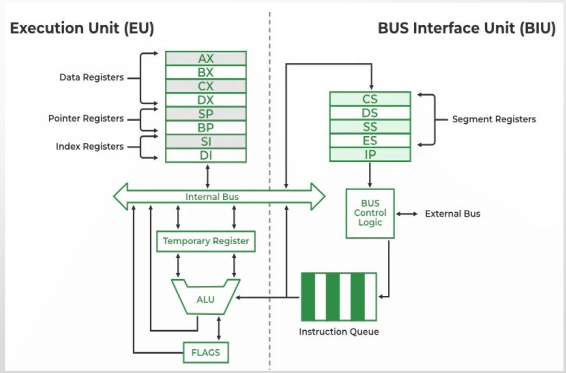
\includegraphics[width=0.5\linewidth]{immagini/introduzione4}
\end{figure}

Per funzionare correttamente, un microprocessore necessita di componenti e risorse circuitali esterne al chip:
\begin{itemize}
    \item Un'ampia memoria volatile di lavoro (RAM esterna) e supporti di memoria di massa (hard disk o memorie a stato solido) per la gestione di grandi quantità di dati.
    \item Interfacce e controller dedicati per periferiche di ingresso (tastiere, puntatori, scanner, microfoni).
    \item Interfacce per dispositivi di uscita (display, monitor, stampanti, attuatori audio).
    \item Potenza di alimentazione elevata, con consumi che possono raggiungere decine o centinaia di watt.
\end{itemize}

\subsubsection{Microcontrollore}
Un microcontrollore (MCU) è un dispositivo di elaborazione dati concettualmente analogo al microprocessore ma basato tipicamente su \textbf{architettura Harvard} (con bus e spazi di memoria separati per istruzioni e dati) e \textbf{set di istruzioni RISC}. L'elemento distintivo fondamentale risiede nell'integrazione monolitica su un unico circuito integrato (single-chip) di tutti i sottosistemi necessari all'elaborazione:
\begin{itemize}
    \item Una CPU RISC.
    \item Una memoria di programma non volatile interna (EPROM, EEPROM o Flash).
    \item Una memoria volatile di lavoro interna (SRAM di dimensioni limitate, da pochi kB a centinaia di kB).
    \item Porte digitali di ingresso e uscita (GPIO).
    \item Timer, contatori hardware e convertitori analogico-digitali (ADC).
    \item Interfacce di comunicazione seriale sincrone e asincrone (UART, SPI, I2C, I2S, RMII, generatori PWM).
\end{itemize}
\begin{figure}[H]
	\centering
	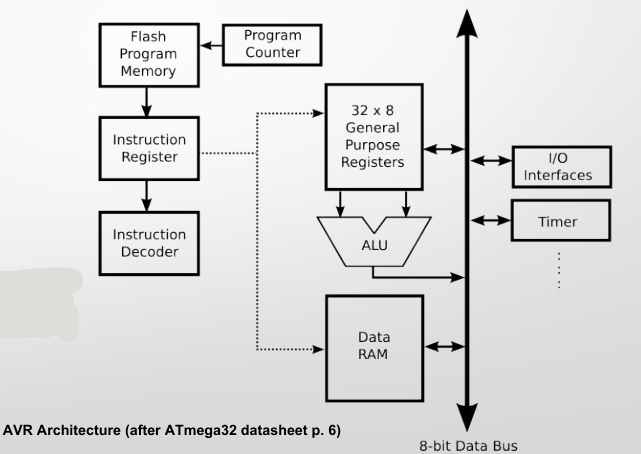
\includegraphics[width=0.6\linewidth]{immagini/introduzione5}
\end{figure}

Mentre i microprocessori costituiscono il nucleo di personal computer, cluster e server, i microcontrollori sono il fondamento dei dispositivi industriali, autronici e domotici. La MCU include sia i componenti base di una CPU (seppure con capacità ridotta) sia una serie di periferiche hardware che il microprocessore non possiede.

\newpage
Il confronto strutturale evidenzia precise divergenze progettuali:
\begin{itemize}
    \item \textbf{Microcontrollore (MCU)}: architettura Harvard e RISC, memorie RAM e Flash integrate internamente sul die, consumi energetici ridotti, basso costo unitario, elevata densità di periferiche on-chip, dotazione hardware nativa per il determinismo Real-Time (controller DMA dedicati, matrici di bus interne senza contesa, gestione interrupt vettorizzata con livelli multipli di priorità e nesting).
    \item \textbf{Microprocessore (MPU)}: architettura Von Neumann e prevalentemente CISC, memorie RAM e ROM collocate esternamente rispetto al die, frequenze di clock elevate, elevatissima potenza di calcolo computazionale, ridotto numero di periferiche integrate on-chip, throughput elevato verso la RAM esterna, molteplici livelli di cache integrata e presenza della MMU.
\end{itemize}

Nelle attuali generazioni di silicio le barriere architetturali tendono a sfumare: esistono microcontrollori avanzati con capacità computazionali assimilabili a microprocessori, microprocessori arricchiti con periferiche integrate (ADC e timer), microcontrollori dotati di cache o bus di espansione verso memorie esterne, e architetture eterogenee multicore (HMP - Heterogeneous Multi-core Processing) che integrano core applicativi MPU e core MCU dedicati al Real-Time sul medesimo silicio.

L'elemento cardine che traccia la reale linea di demarcazione tra microprocessori e microcontrollori è la presenza o l'assenza della \textbf{MMU (Memory Management Unit)}.

La MMU costituisce il blocco circuitale indispensabile per consentire l'esecuzione di un sistema operativo General-Purpose moderno. Le sue funzioni primarie includono:
\begin{itemize}
    \item \textbf{Virtualizzazione degli indirizzi} $\rightarrow$ conversione degli indirizzi di memoria virtuali generati dai processi software negli effettivi indirizzi fisici della memoria RAM.
    \item \textbf{Protezione della memoria} $\rightarrow$ impedisce a singoli processi di accedere senza autorizzazione alla memoria di altri processi o allo spazio riservato del kernel.
    \item \textbf{Gestione della frammentazione} $\rightarrow$ ricomposizione logica di pagine allocate in modo frammentato nella memoria fisica, garantendo allo spazio utente la visibilità di un'area di memoria perfettamente contigua e massimizzando lo sfruttamento dello spazio.
    \item \textbf{Controllo della cache} $\rightarrow$ supervisione delle politiche di allocazione della memoria cache e mantenimento della coerenza dei dati tra cache e memoria centrale.
    \item \textbf{Arbitraggio del bus} $\rightarrow$ regolamentazione e prioritizzazione degli accessi concorrenti ai bus dati e indirizzi tra CPU e periferiche master.
    \item \textbf{Gestione dei banchi di memoria} $\rightarrow$ coordinamento e selezione dinamica dei differenti moduli e banchi costituenti il sottosistema di memoria.
\end{itemize}

\textbf{Nei microcontrollori tradizionali la MMU è assente}, poiché il meccanismo di virtualizzazione e rilocazione delle pagine introduce latenze non prevedibili, incompatibili con i requisiti di determinismo temporale tipici dei sistemi embedded e Real-Time.

Un'altra differenza fondamentale tra microprocessori e microcontrollori è sulle \textbf{taglie di memoria}, che differiscono sistematicamente di almeno due ordini di grandezza:
\begin{itemize}
    \item \textbf{Memoria Volatile (RAM)}:
    \begin{itemize}
        \item MCU RAM interna $\rightarrow$ da pochi kB fino a un limite massimo di circa 1 MB, con valori tipici compresi nell'ordine delle centinaia di kB.
        \item MCU RAM esterna $\rightarrow$ moduli opzionali espandibili da 64 MB fino a 512 MB o 1 GB.
        \item MPU RAM $\rightarrow$ configurazioni standard su banchi esterni pari a 16 GB o 32 GB.
    \end{itemize}
    \newpage
    \item \textbf{Memoria Non Volatile (Flash e Storage)}:
    \begin{itemize}
        \item MCU Flash interna $\rightarrow$ da poche decine di kB fino a 2 MB per la memorizzazione permanente del firmware.
        \item MCU Flash esterna $\rightarrow$ memorie collegate tramite interfacce ad alta velocità (es. QSPI) estendibili fino a qualche GB.
        \item MPU Mass Storage $\rightarrow$ memorie di massa secondarie con capacità nell'ordine di 2 TB o superiori.
    \end{itemize}
\end{itemize}

\section{Architetture Software per Sistemi Embedded}
La realizzazione del software nei sistemi embedded si fonda su tre principali paradigmi operativi: il modello ciclico Foreground-Background, i sistemi operativi Real-Time (RTOS) e le distribuzioni Linux Embedded.

\subsubsection{Foreground-background}
Nel modello Foreground-Background (superloop con interruzioni), l'esecuzione è strutturata su due livelli di priorità:
\begin{itemize}
    \item \textbf{Background} $\rightarrow$ costituito dalla funzione ciclica \texttt{main()}, un ciclo infinito in cui vengono eseguite in sequenza le attività a bassa priorità, le elaborazioni non critiche e la manutenzione ordinaria dello stato del sistema.
    \item \textbf{Foreground} $\rightarrow$ costituito dalle Routine di Servizio delle Interruzioni (\textbf{ISR}), richiamate asincronamente al manifestarsi di segnali di interrupt hardware (\textbf{IRQ}) generati dalle periferiche o dall'esterno. Le ISR sospendono l'esecuzione del ciclo di background per gestire immediatamente gli eventi prioritari e urgenti, restituendo quindi il controllo al punto interrotto mediante l'istruzione di ritorno da interruzione (\textbf{rti}).
\end{itemize}
\begin{figure}[H]
	\centering
	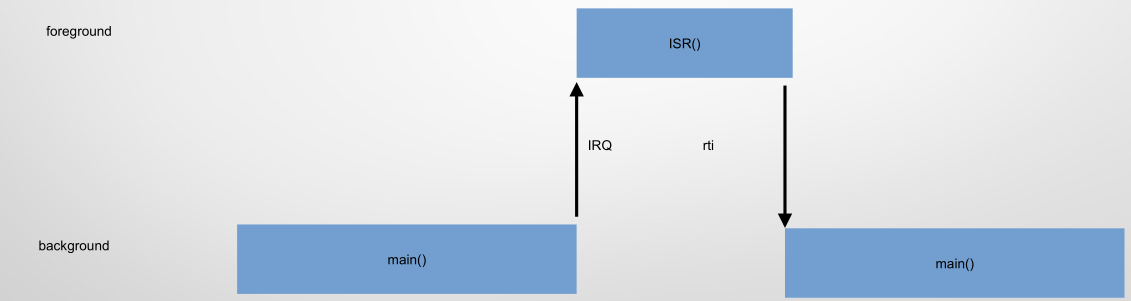
\includegraphics[width=0.9\linewidth]{immagini/introduzione6}
\end{figure}

\subsubsection{Sistemi operativi Real-Time (RTOS)}
Nei contesti a complessità superiore si impiegano gli RTOS (Real-Time Operating System), sistemi operativi minimali a bassissimo footprint di memoria sviluppati appositamente per microcontrollori. Le loro peculiarità includono:
\begin{itemize}
    \item Assenza della gestione dinamica della memoria, evitata per scongiurare fenomeni di frammentazione dell'heap e garantire tempi di allocazione deterministici.
    \item Presenza di politiche di scheduling tassativamente concepite per garantire la certezza dei tempi di esecuzione dei task.
    \newpage
    \item Meccanismi di arbitraggio dell'elaborazione basati su:
    \begin{itemize}
    	\item \textbf{Scheduling cooperativo Round Robin} $\rightarrow$ suddivisione equa del tempo di CPU tra processi di pari livello.
    	\begin{figure}[H]
    		\centering
    		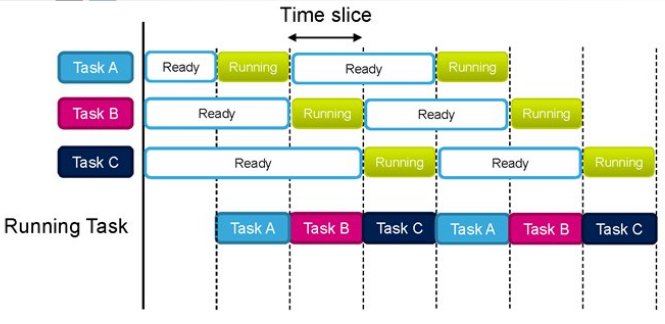
\includegraphics[width=0.55\linewidth]{immagini/introduzione8}
    	\end{figure}
    	\item \textbf{Scheduling preemptive Priority-based} $\rightarrow$ prelazione immediata della CPU a favore del task a priorità superiore.
    	\begin{figure}[H]
    		\centering
    		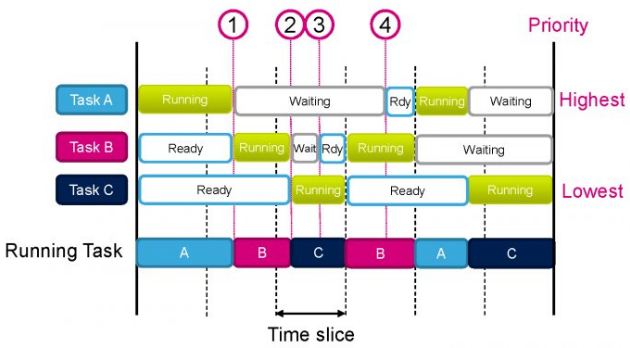
\includegraphics[width=0.55\linewidth]{immagini/introduzione9}
    	\end{figure}
    \end{itemize}
\end{itemize}
\textbf{NOTA}: nelle applicazioni embedded si usa spesso, in modo improprio, il termine \textbf{task}. In realtà si tratta di \textbf{thread}, non di task. Entrambi indicano flussi di operazioni, ma con una differenza fondamentale: i thread condividono la stessa memoria, mentre i task no. Nei sistemi basati su RTOS, quindi, il termine corretto è thread.

\subsubsection{Linux Embedded}
L'architettura software di un sistema operativo embedded differisce radicalmente da quella di un sistema operativo convenzionale General-Purpose:
\begin{itemize}
    \item Nel \textbf{sistema operativo General-Purpose}, al di sopra del kernel e del gestore del caricamento (OS Loader) risiedono componenti pesanti quali il file system, il controllo del disco e l'interfaccia utente grafica (OS User Interface Shell), preposti a lanciare ed eseguire una moltitudine di programmi applicativi indipendenti.
    \item Nel \textbf{sistema operativo embedded}, l'architettura è snella: al di sopra dell'hardware e del kernel risiedono esclusivamente l'OS Loader e i moduli di interfacciamento con il mondo fisico reale (Real-world interfaces), direttamente asserviti alla singola applicazione dedicata.
\end{itemize}
\begin{figure}[H]
	\centering
	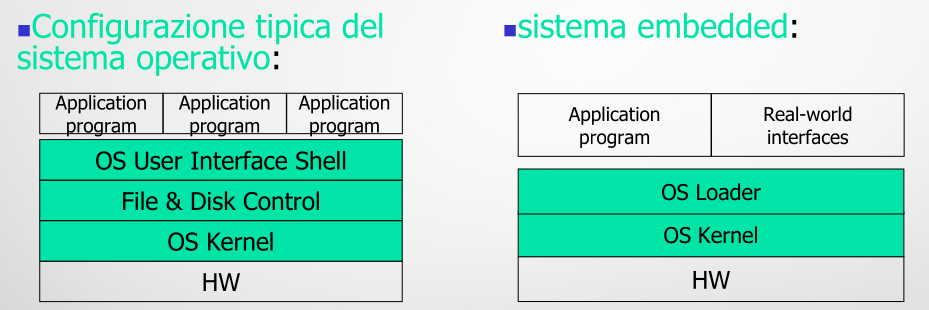
\includegraphics[width=0.5\linewidth]{immagini/introduzione10}
\end{figure}

Per sistemi basati su System-on-Chip (SoC) o Application Processor complessi trova impiego Linux Embedded. Trattandosi di un sistema operativo open-source universale sostenuto da un'ampia comunità internazionale e dal settore industriale, Linux consente di configurare e compilare su misura sia il kernel sia l'intera distribuzione, eliminando tutti i servizi non necessari e riducendo l'impronta di memoria ai minimi requisiti dell'applicazione.

Il principale beneficio dell'approccio Linux risiede nella possibilità di integrare agevolmente moduli e librerie software open-source preesistenti, accelerando lo sviluppo applicativo. Tuttavia, il kernel Linux convenzionale non presenta caratteristiche Real-Time native; per ottenere determinismo si ricorre alla patch Real-Time di Linux (PREEMPT\_RT), estesamente adottata in contesti avanzati di robotica e intelligenza artificiale. Linux Real-Time assicura un comportamento rigorosamente prevedibile, garantendo che le attività a priorità critica ricevano immediata attenzione ed esecuzione entro scadenze temporali vincolanti. Sistemi operativi commerciali proprietari per PC (come Windows) risultano invece inadatti per applicazioni embedded critiche a causa della suscettibilità a blocchi sistemici imprevisti (es. schermate blu di errore / BSOD) e dell'assenza di determinismo temporale.

I sistemi operativi Linux embedded trovano largo impiego nel mondo degli apparati di rete (router, acces point, ecc...) con \textit{OpenWrt}, bilance elettroniche, TV box (\textit{Dreambox}), automazione industriale e acquisizione dati (\textit{National Instruments CompactRIO}), domotica e smart home (\textit{Google Nest}), gaming e console portatili (\textit{Nintendo Switch}) e tanto altro ancora.
\begin{figure}[H]
	\centering
	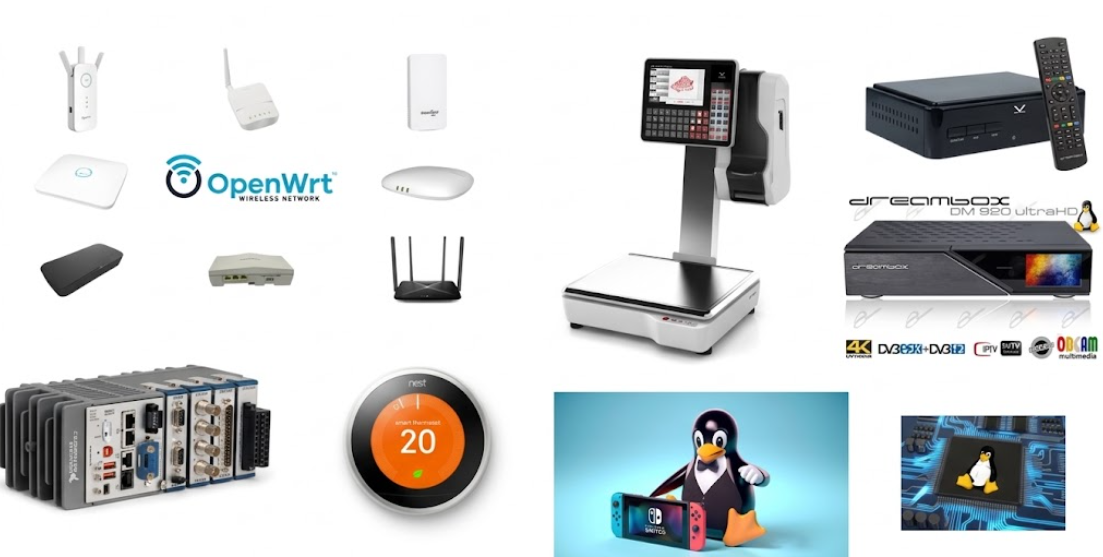
\includegraphics[width=0.8\linewidth]{immagini/introduzione11}
\end{figure}

\newpage
\section{Prototipazione rapida e ingegnerizzazione}
L'evoluzione dell'elettronica digitale ha reso la tecnologia contemporaneamente sempre più complessa e sempre più accessibile. Piattaforme hardware modulari di Rapid Prototyping hanno abilitato la nascita del movimento dei \textbf{Maker}, consentendo a progettisti e hobbisti di sperimentare soluzioni innovative e introdurre rapidamente l'elettronica in ambiti inediti.

Le piattaforme di prototipazione rapida maggiormente diffuse si ripartiscono in due categorie tecnologiche distinte:
\begin{itemize}
    \item \textbf{Arduino} $\rightarrow$ soluzione embedded incentrata su firmware puro, basata su architettura a microcontrollore e orientata al controllo diretto di I/O fisici.
    \item \textbf{Raspberry Pi} $\rightarrow$ soluzione Linux embedded incentrata su microprocessore e architettura SoC, orientata ad applicazioni complesse ad alto livello di astrazione.
\end{itemize}
\begin{figure}[H]
	\centering
	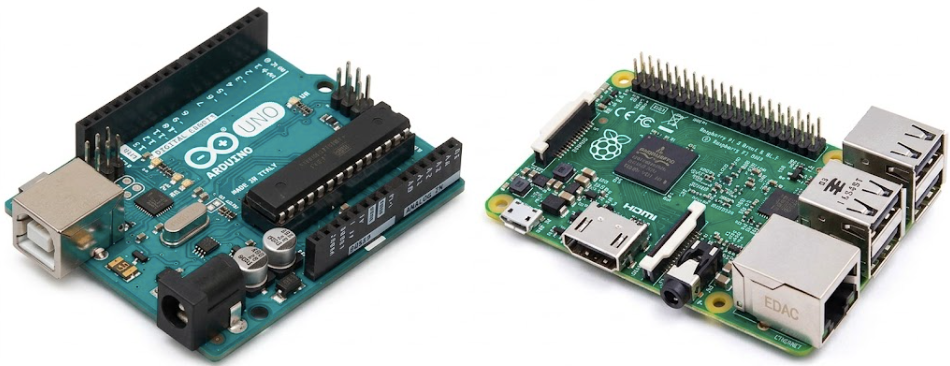
\includegraphics[width=0.5\linewidth]{immagini/introduzione12}
\end{figure}


Sebbene l'uso di piattaforme rapide faciliti lo sviluppo iniziale grazie alla disponibilità di librerie, driver e schede di espansione preassemblate, sussiste una differenza fondamentale tra un approccio hobbistico o amatoriale e un approccio ingegneristico professionale:
\begin{itemize}
    \item Un \textbf{prototipo} (Proof of Concept) rappresenta una validazione concettuale di laboratorio. Non è progettato per durare nel tempo e opera unicamente nelle condizioni ambientali migliori possibili (Best Case).
    \item Un \textbf{prodotto finito} deve essere interamente ingegnerizzato, rispettando la totalità dei requisiti di affidabilità, compattezza, sicurezza e conformità normativa fissati per i sistemi embedded.
\end{itemize}

L'ambiente reale in cui il prodotto embedded è chiamato a operare è intrinsecamente severo e ostile. Un'ingegnerizzazione rigorosa impone il passaggio fondamentale dalla progettazione nominale alla progettazione per il caso peggiore (Worst Case Design), fronteggiando molteplici condizioni avverse:
\begin{itemize}
    \item Escursioni termiche ambientali estreme.
    \item Presenza di contaminanti atmosferici, polvere e particolato.
    \item Umidità elevata e condense corrosive.
    \item Sollecitazioni meccaniche continuative e vibrazioni.
    \item Interferenze elettromagnetiche (EMI/EMC) e disturbi indotti sulle linee di segnale e alimentazione.
    \item Utilizzo improprio, manomissione o errori da parte dell'utente finale.
\end{itemize}

La transizione verso un prodotto professionale richiede la piena padronanza dei fondamenti teorici e dei limiti fisici del mondo reale:
\begin{itemize}
    \item I componenti fisici presentano \textbf{limiti operativi stringenti}; ad esempio, la lunghezza dei collegamenti via cavo (cable length) incide su attenuazione, cadute di tensione, ritardi di propagazione e accoppiamenti parassiti.
    \item Obbligo di conformità e rispetto delle \textbf{norme tecniche}, degli standard industriali e delle direttive legislative e di sicurezza vigenti.
    \item Svolgimento degli iter di collaudo e acquisizione delle \textbf{certificazioni obbligatorie} di prodotto.
\end{itemize}

La sottovalutazione dei vincoli ambientali, l'impiego di prototipi non ingegnerizzati o la presenza di difetti di progettazione nell'hardware e nel firmware possono determinare guasti disastrosi. Nel contesto dei sistemi embedded industriali e mission-critical, un piccolo errore progettuale comporta costi economici estremamente elevati e rischi inaccettabili per la sicurezza.
